\section*{Supplementary Material}

% Create new counter for supplement sections
\newcounter{suppsection}
\newcounter{suppsubsection}[suppsection]

% Configure supplement numbering
\renewcommand{\thesuppsection}{S\arabic{suppsection}}
\renewcommand{\thesuppsubsection}{\thesuppsection.\arabic{suppsubsection}}

% Reset counters for supplement
\setcounter{table}{0}
\setcounter{figure}{0}

% Configure table and figure numbering
\renewcommand{\thetable}{S\arabic{table}}
\renewcommand{\thefigure}{S\arabic{figure}}

% Reset and configure page numbering
\setcounter{page}{1}
\renewcommand{\thepage}{S\arabic{page}}

% Define supplement section command
\newcommand{\suppsection}[1]{%
  \refstepcounter{suppsection}%
  \section*{S\arabic{suppsection}. #1}\label{supp:\arabic{suppsection}}%
}

% Define supplement subsection command
\newcommand{\suppsubsection}[1]{%
  \refstepcounter{suppsubsection}%
  \subsection*{S\arabic{suppsection}.\arabic{suppsubsection}. #1}\label{supp:\arabic{suppsection}.\arabic{suppsubsection}}%
}

\suppsection{Data Harvesting Implementation}\label{supp:data_harvesting}

Our data harvesting system employs DuckDB for efficient querying of PARQUET files, enabling complex joins and aggregations without full memory loading. For species matching across databases, we use structured SQL queries that join on concatenated genus and species names:

\begin{verbatim}
SELECT 
    SpecCode, PreySpecCode, AlphaCode, 
    Foodgroup, Foodname, PreyStage, PredatorStage, FoodI, FoodII, FoodIII, 
    Commoness, CommonessII, PreyTroph, PreySeTroph
FROM sealifebase_df
WHERE SpecCode IN ({','.join(map(str, valid_codes))})
AND (PreyStage LIKE '%adult%' OR PreyStage LIKE '%juv%')
AND (PredatorStage LIKE '%adult%' OR PredatorStage LIKE '%juv%')
\end{verbatim}

When combining interaction data from GLOBI with diet information, we implement a comprehensive interaction mapping system that creates bidirectional records:

\begin{verbatim}
interaction_data[source_group]['preys_on'][target_group] = count
interaction_data[target_group]['is_preyed_on_by'][source_group] = count
\end{verbatim}

Our data cleaning protocol standardises types by converting numerical values to consistent formats and timestamps to ISO format. We handle null values by removing empty values, `NA' strings, and null entries while preserving data structure. Source tracking maintains database origin information for all data points.

The system implements file locking mechanisms for concurrent access, with separate locks for species data and interaction networks. We use exponential backoff retry logic for API interactions, with configurable parameters including maximum retries (5), initial delay (1 second), and maximum delay (60 seconds).

The completion check system verifies the presence of required fields including:
\begin{itemize}
\item Complete taxonomic hierarchy
\item Species-specific database records (when available)
\item Interaction data
\item Source attribution
\item Data quality indicators
\end{itemize}

The final JSON output maintains a consistent structure across all species entries, facilitating automated processing in subsequent framework stages.

\suppsection{Diet Matrix Analysis}\label{supp:diet_matrix}


\begin{landscape}
  \begin{figure}[p]
      \centering
      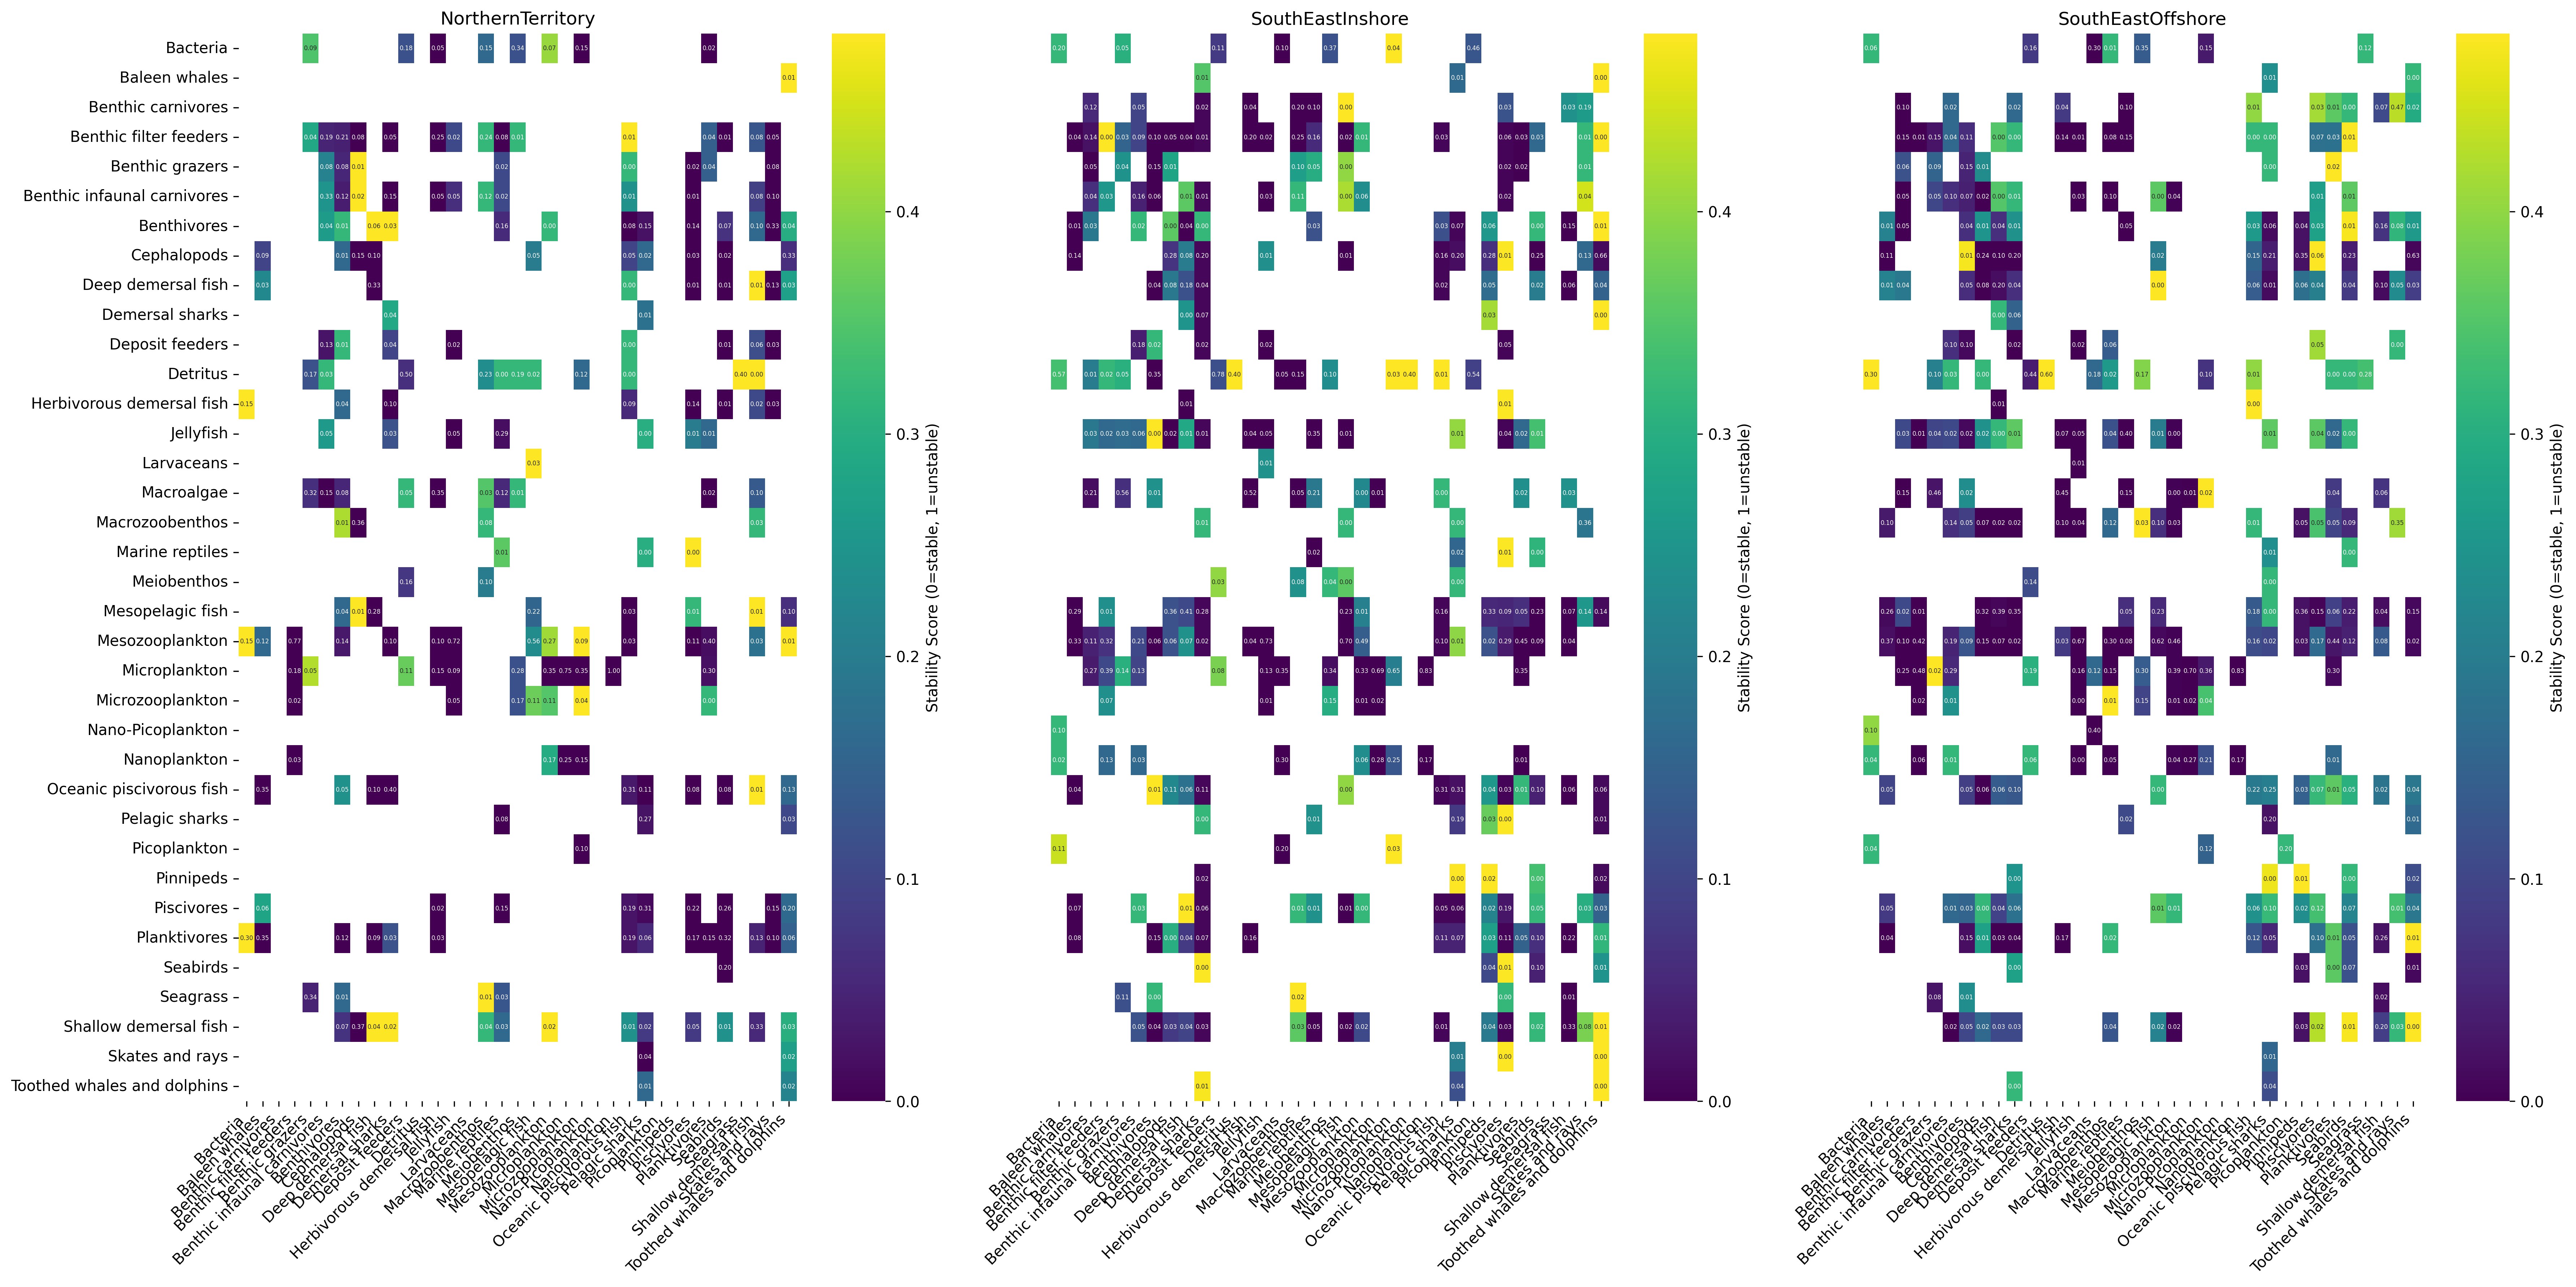
\includegraphics[width=\linewidth]{figures/diet_interaction_heatmap.png}
      \caption{Detailed diet matrix consistency across five iterations for each geographic region. Column names represent predator groups and row names represent their prey groups. Numbers in each cell indicate the mean diet proportions across five iterations, while cell colors indicate the stability score (0-1, where 0 represents perfect stability and 1 represents maximum variation). White cells represent absent feeding relationships. This comprehensive visualization complements the stability score distributions and predator-specific analyses presented in the main text (Figures 4 and 5).}
      \label{fig:diet_matrix_supp}
  \end{figure}
  \end{landscape}

\begin{landscape}
  \begin{figure}[p]
      \centering
      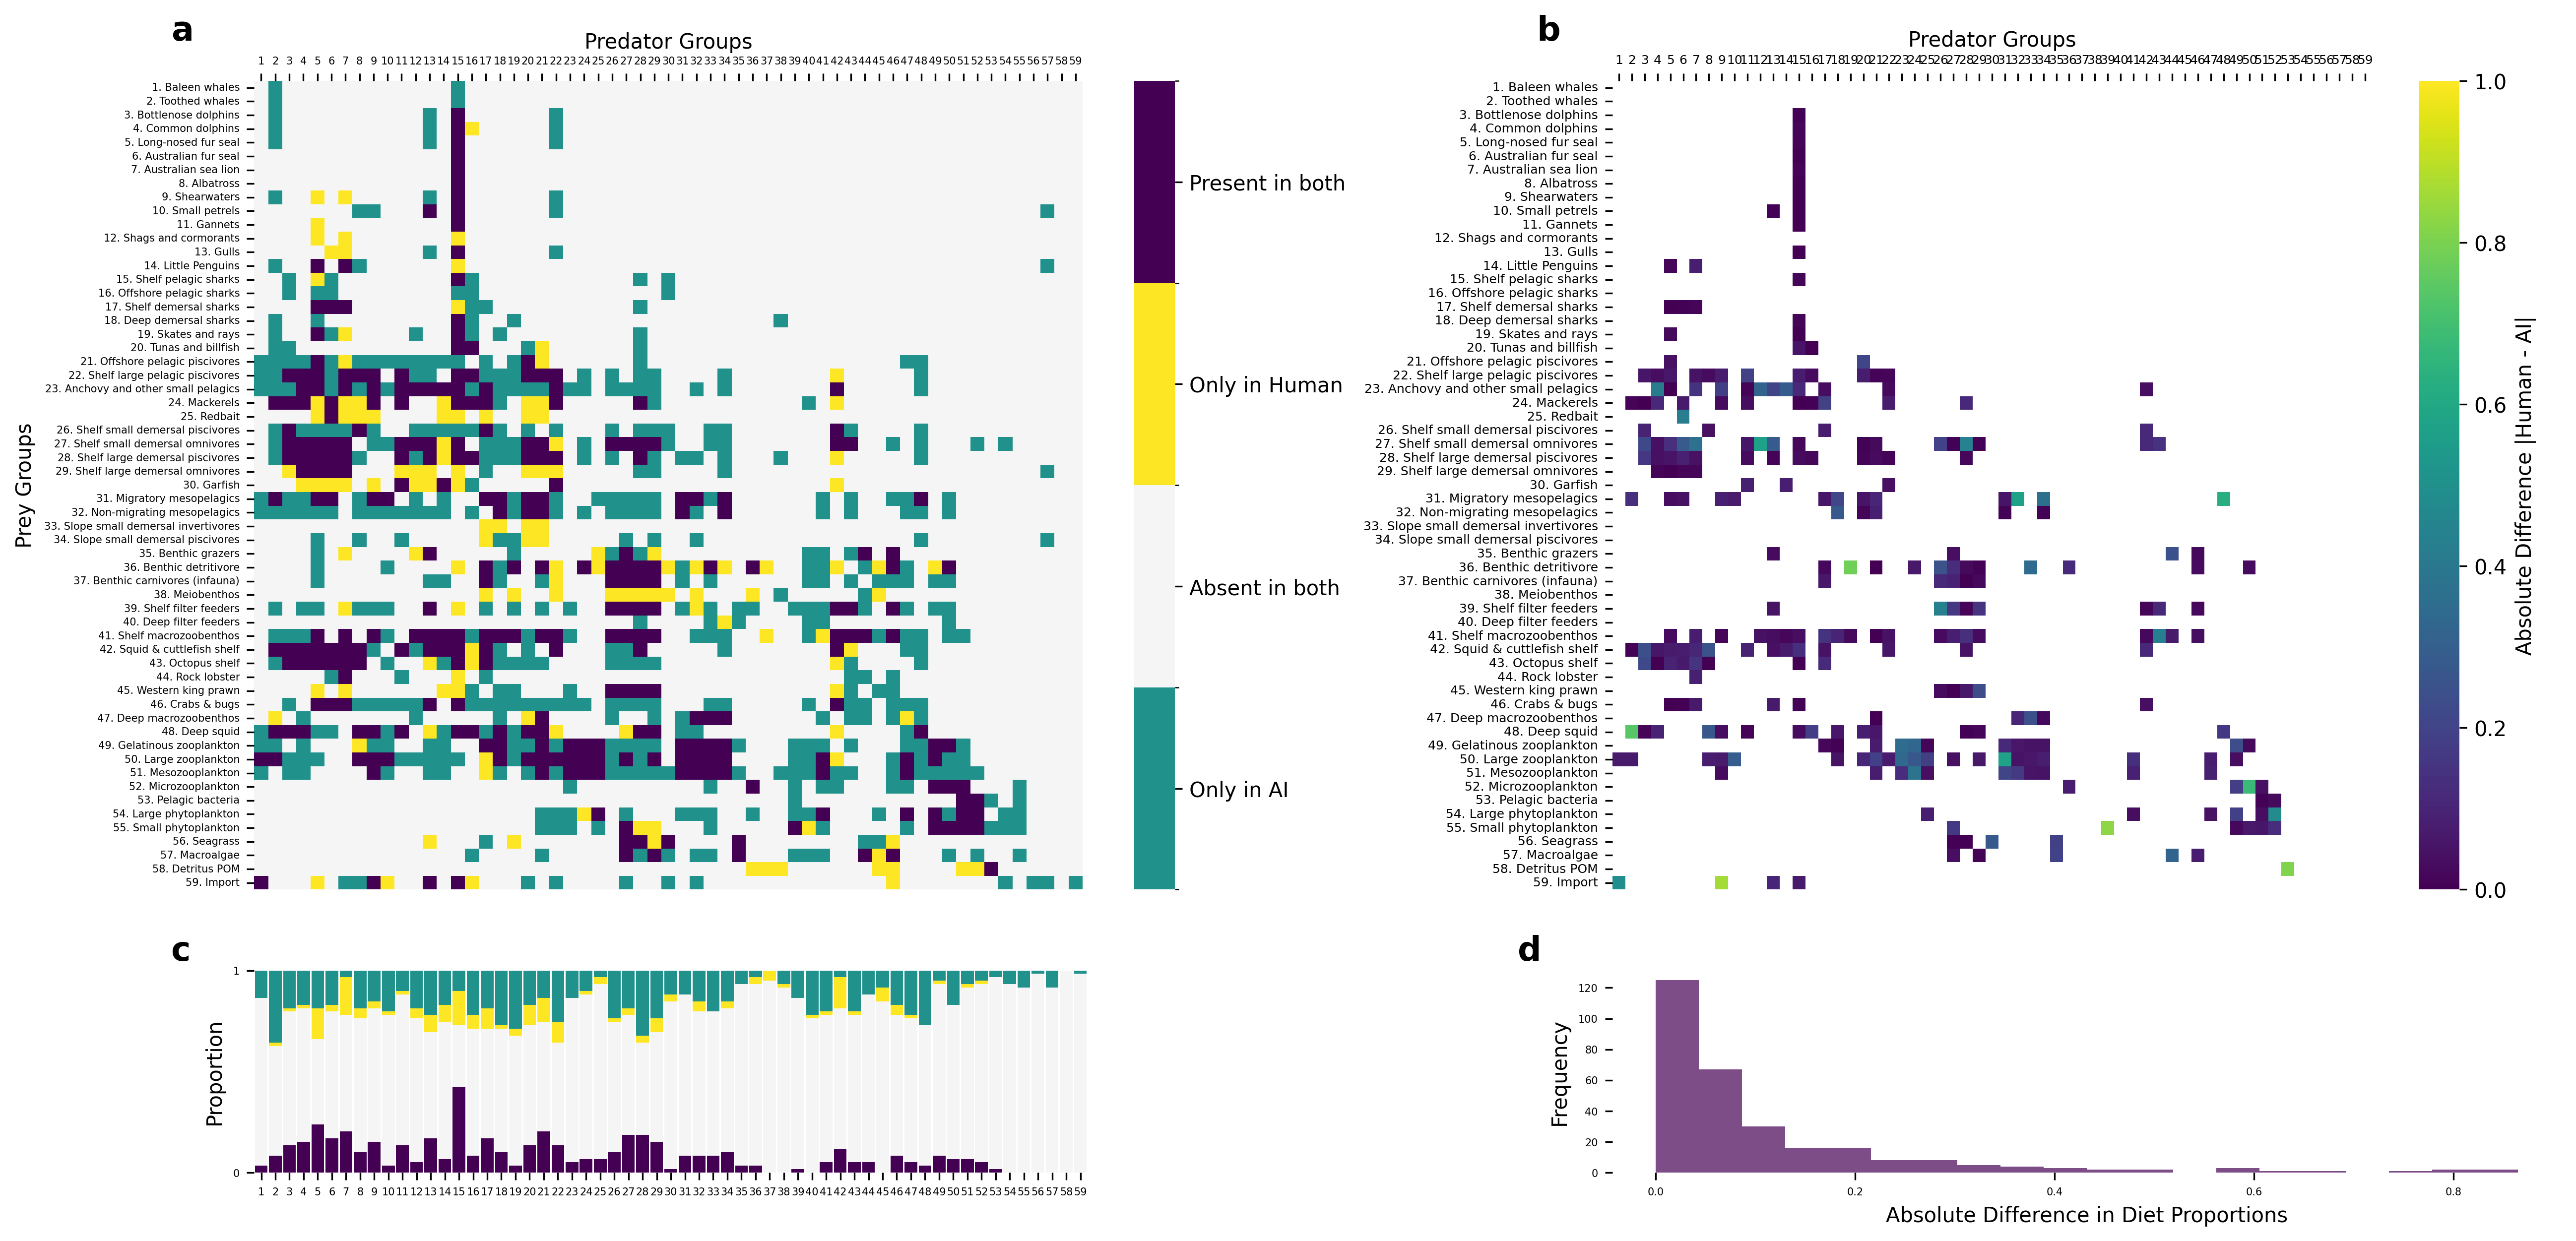
\includegraphics[width=\linewidth]{figures/diet_matrix_validation/detailed_comparison.png}
      \caption{Detailed comparison of diet matrix elements between expert-derived and AI-generated matrices for the Great Australian Bight ecosystem. Panel (a) shows the complete diet matrix with color-coded interaction types: dark purple indicates interactions present in both matrices, yellow shows expert-only interactions, teal shows AI-only interactions, and light grey indicates absence in both. Panel (b) displays the absolute differences in diet proportions between expert and AI matrices where interactions are present in both, with colors ranging from purple (small differences) to yellow (large differences). Panel (c) shows the proportional breakdown of interaction types for each predator group, while panel (d) presents the frequency distribution of absolute differences in diet proportions. This comprehensive visualization expands on Figure \ref{fig:gab_comparison} from the main text by providing a detailed view of each predator-prey relationship and quantifying the differences between expert and AI assessments.}
      \label{fig:detailed_comparison_supp}
  \end{figure}
\end{landscape}
  
\suppsection{Group Stability Analysis}\label{supp:group_stability}

\begin{figure}[htbp]
    \centering
    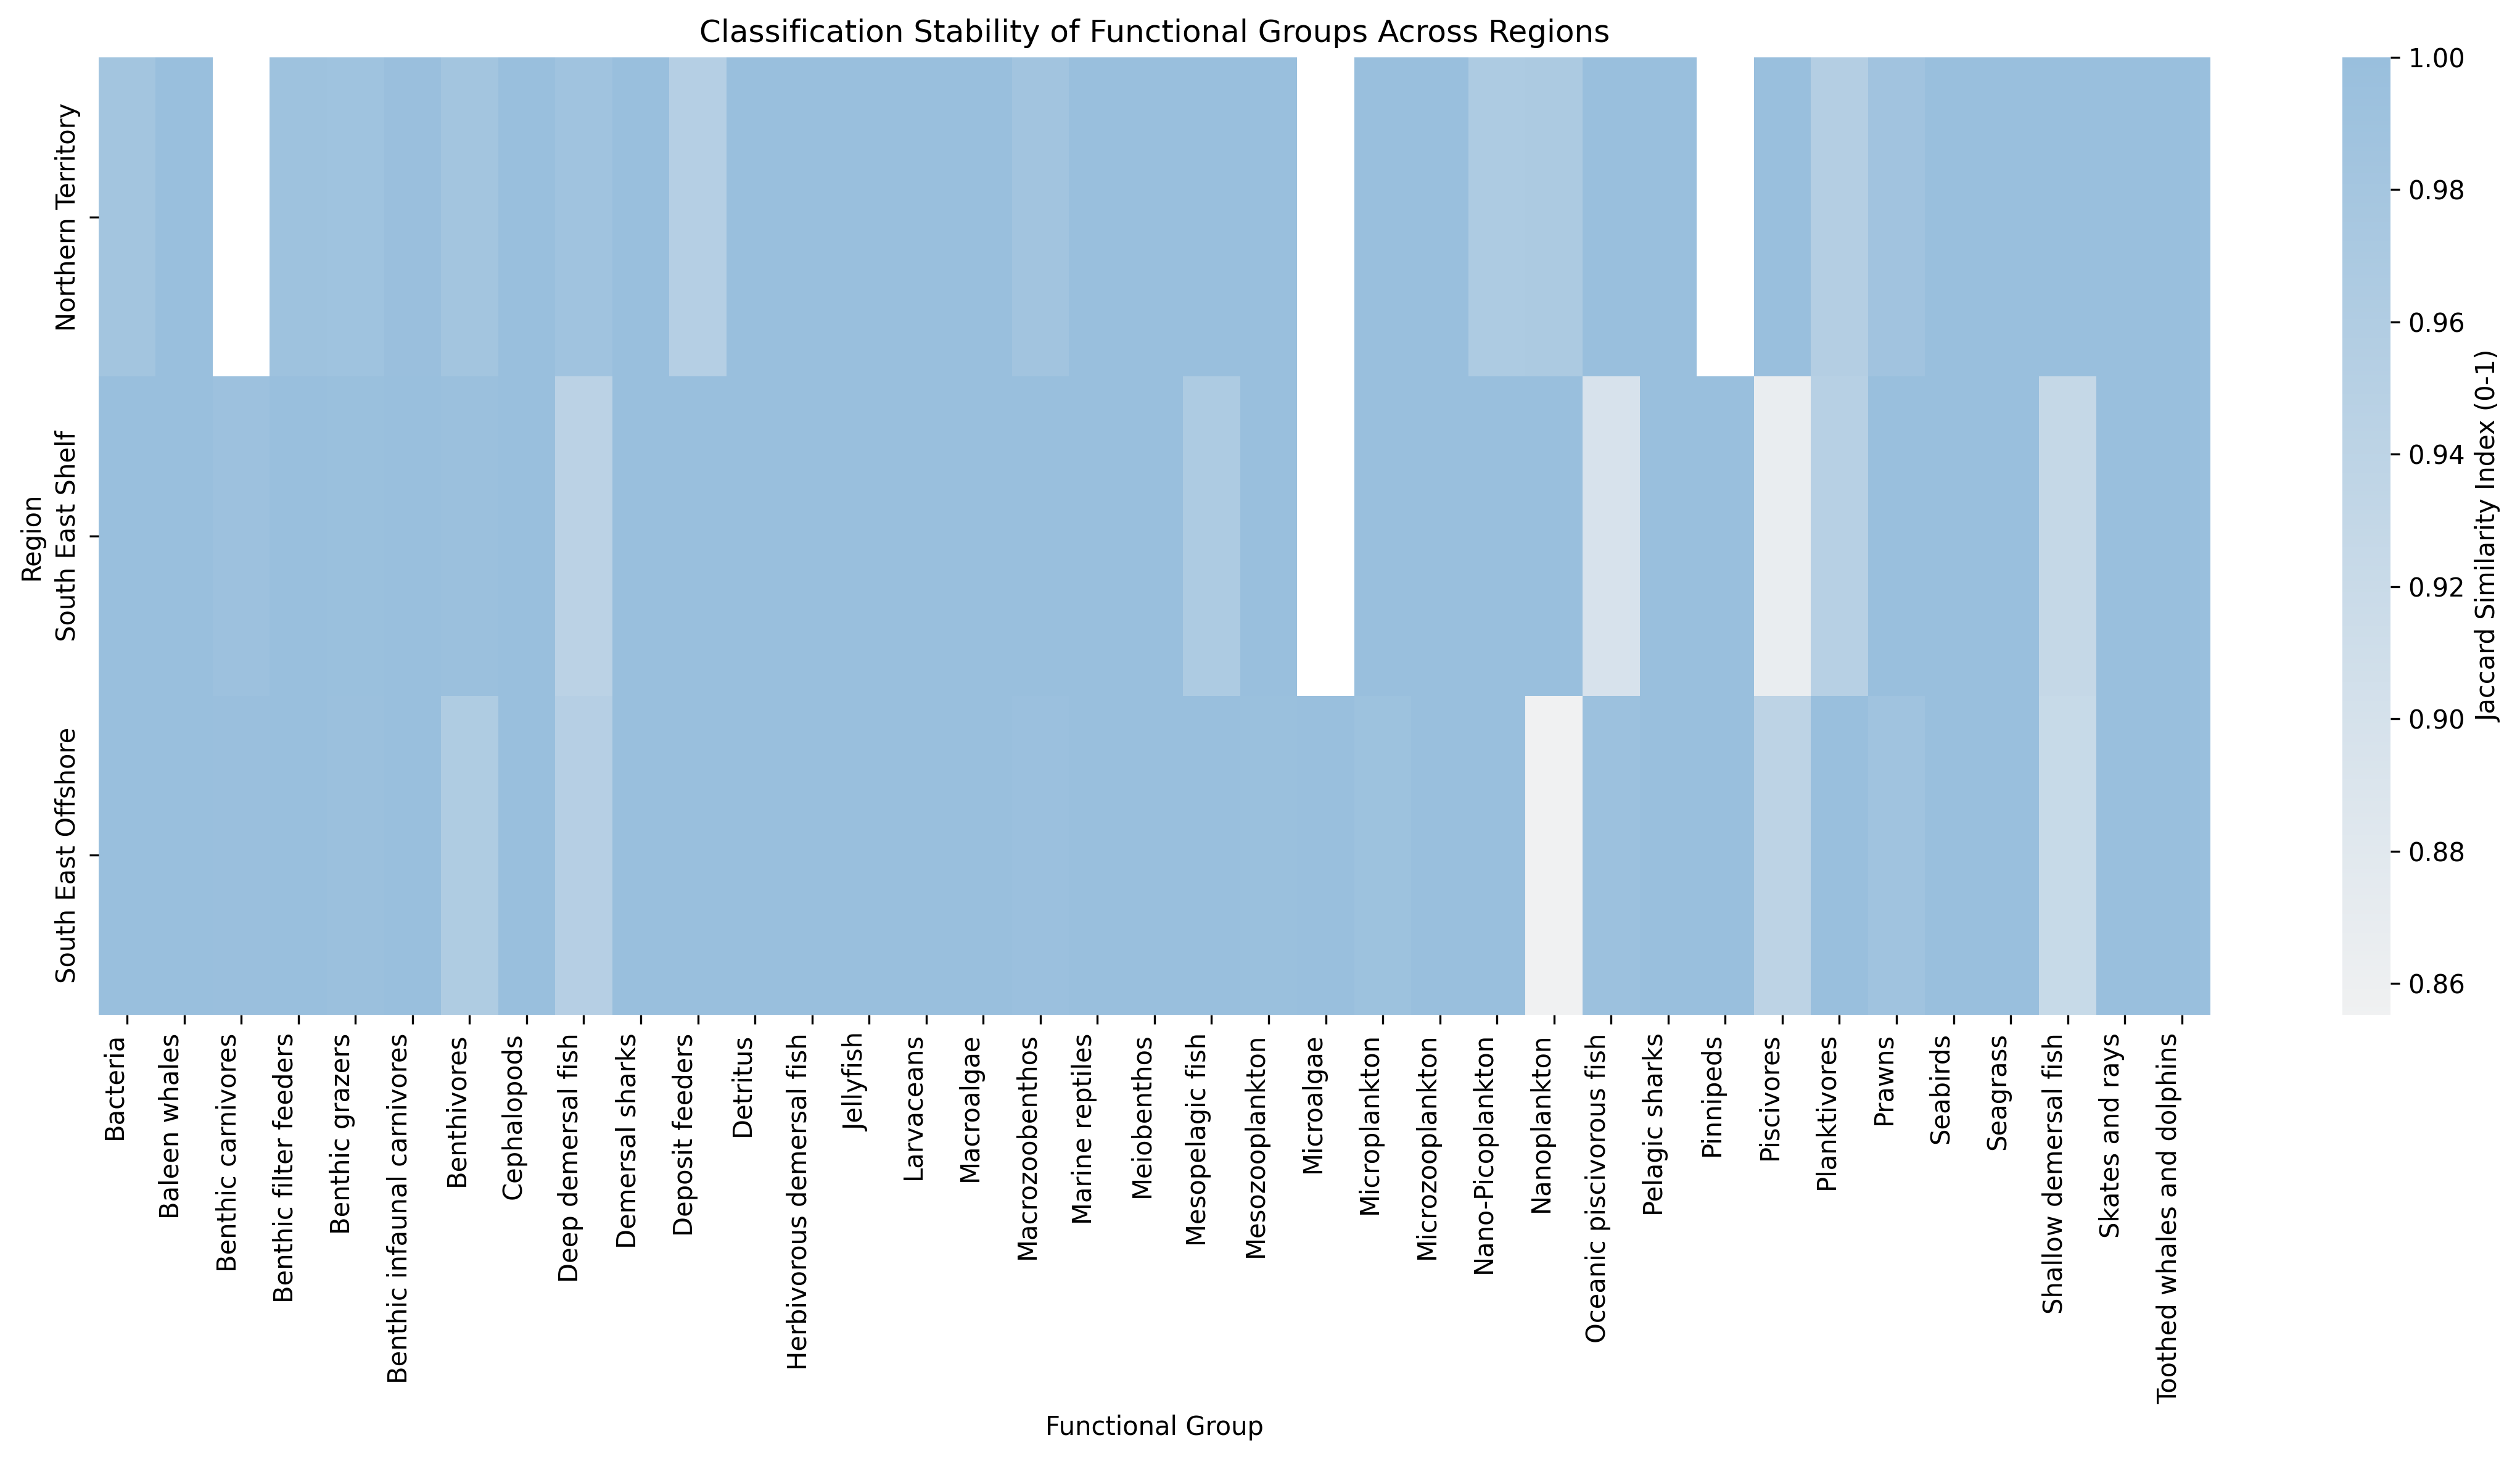
\includegraphics[width=\textwidth]{figures/group_stability_heatmap.png}
    \caption{Heatmap showing the stability of functional group classifications across regions. Each cell displays the Jaccard similarity score (ranging from 0.975 to 1.000) between consecutive framework iterations, where 1.000 indicates perfect consistency in species assignments. Yellow colors represent higher stability (scores near 1.000), while darker purple colors indicate more variable classifications (scores closer to 0.975). Most functional groups show high stability (>0.99) across all regions, with occasional variations in groups like benthic grazers and deposit feeders, particularly in the Northern Australia region. White indicates groups that were not assigned by the AI system for that region.}
    \label{fig:stability_heatmap_supp}
\end{figure}

\begin{figure}[htbp]
  \centering
  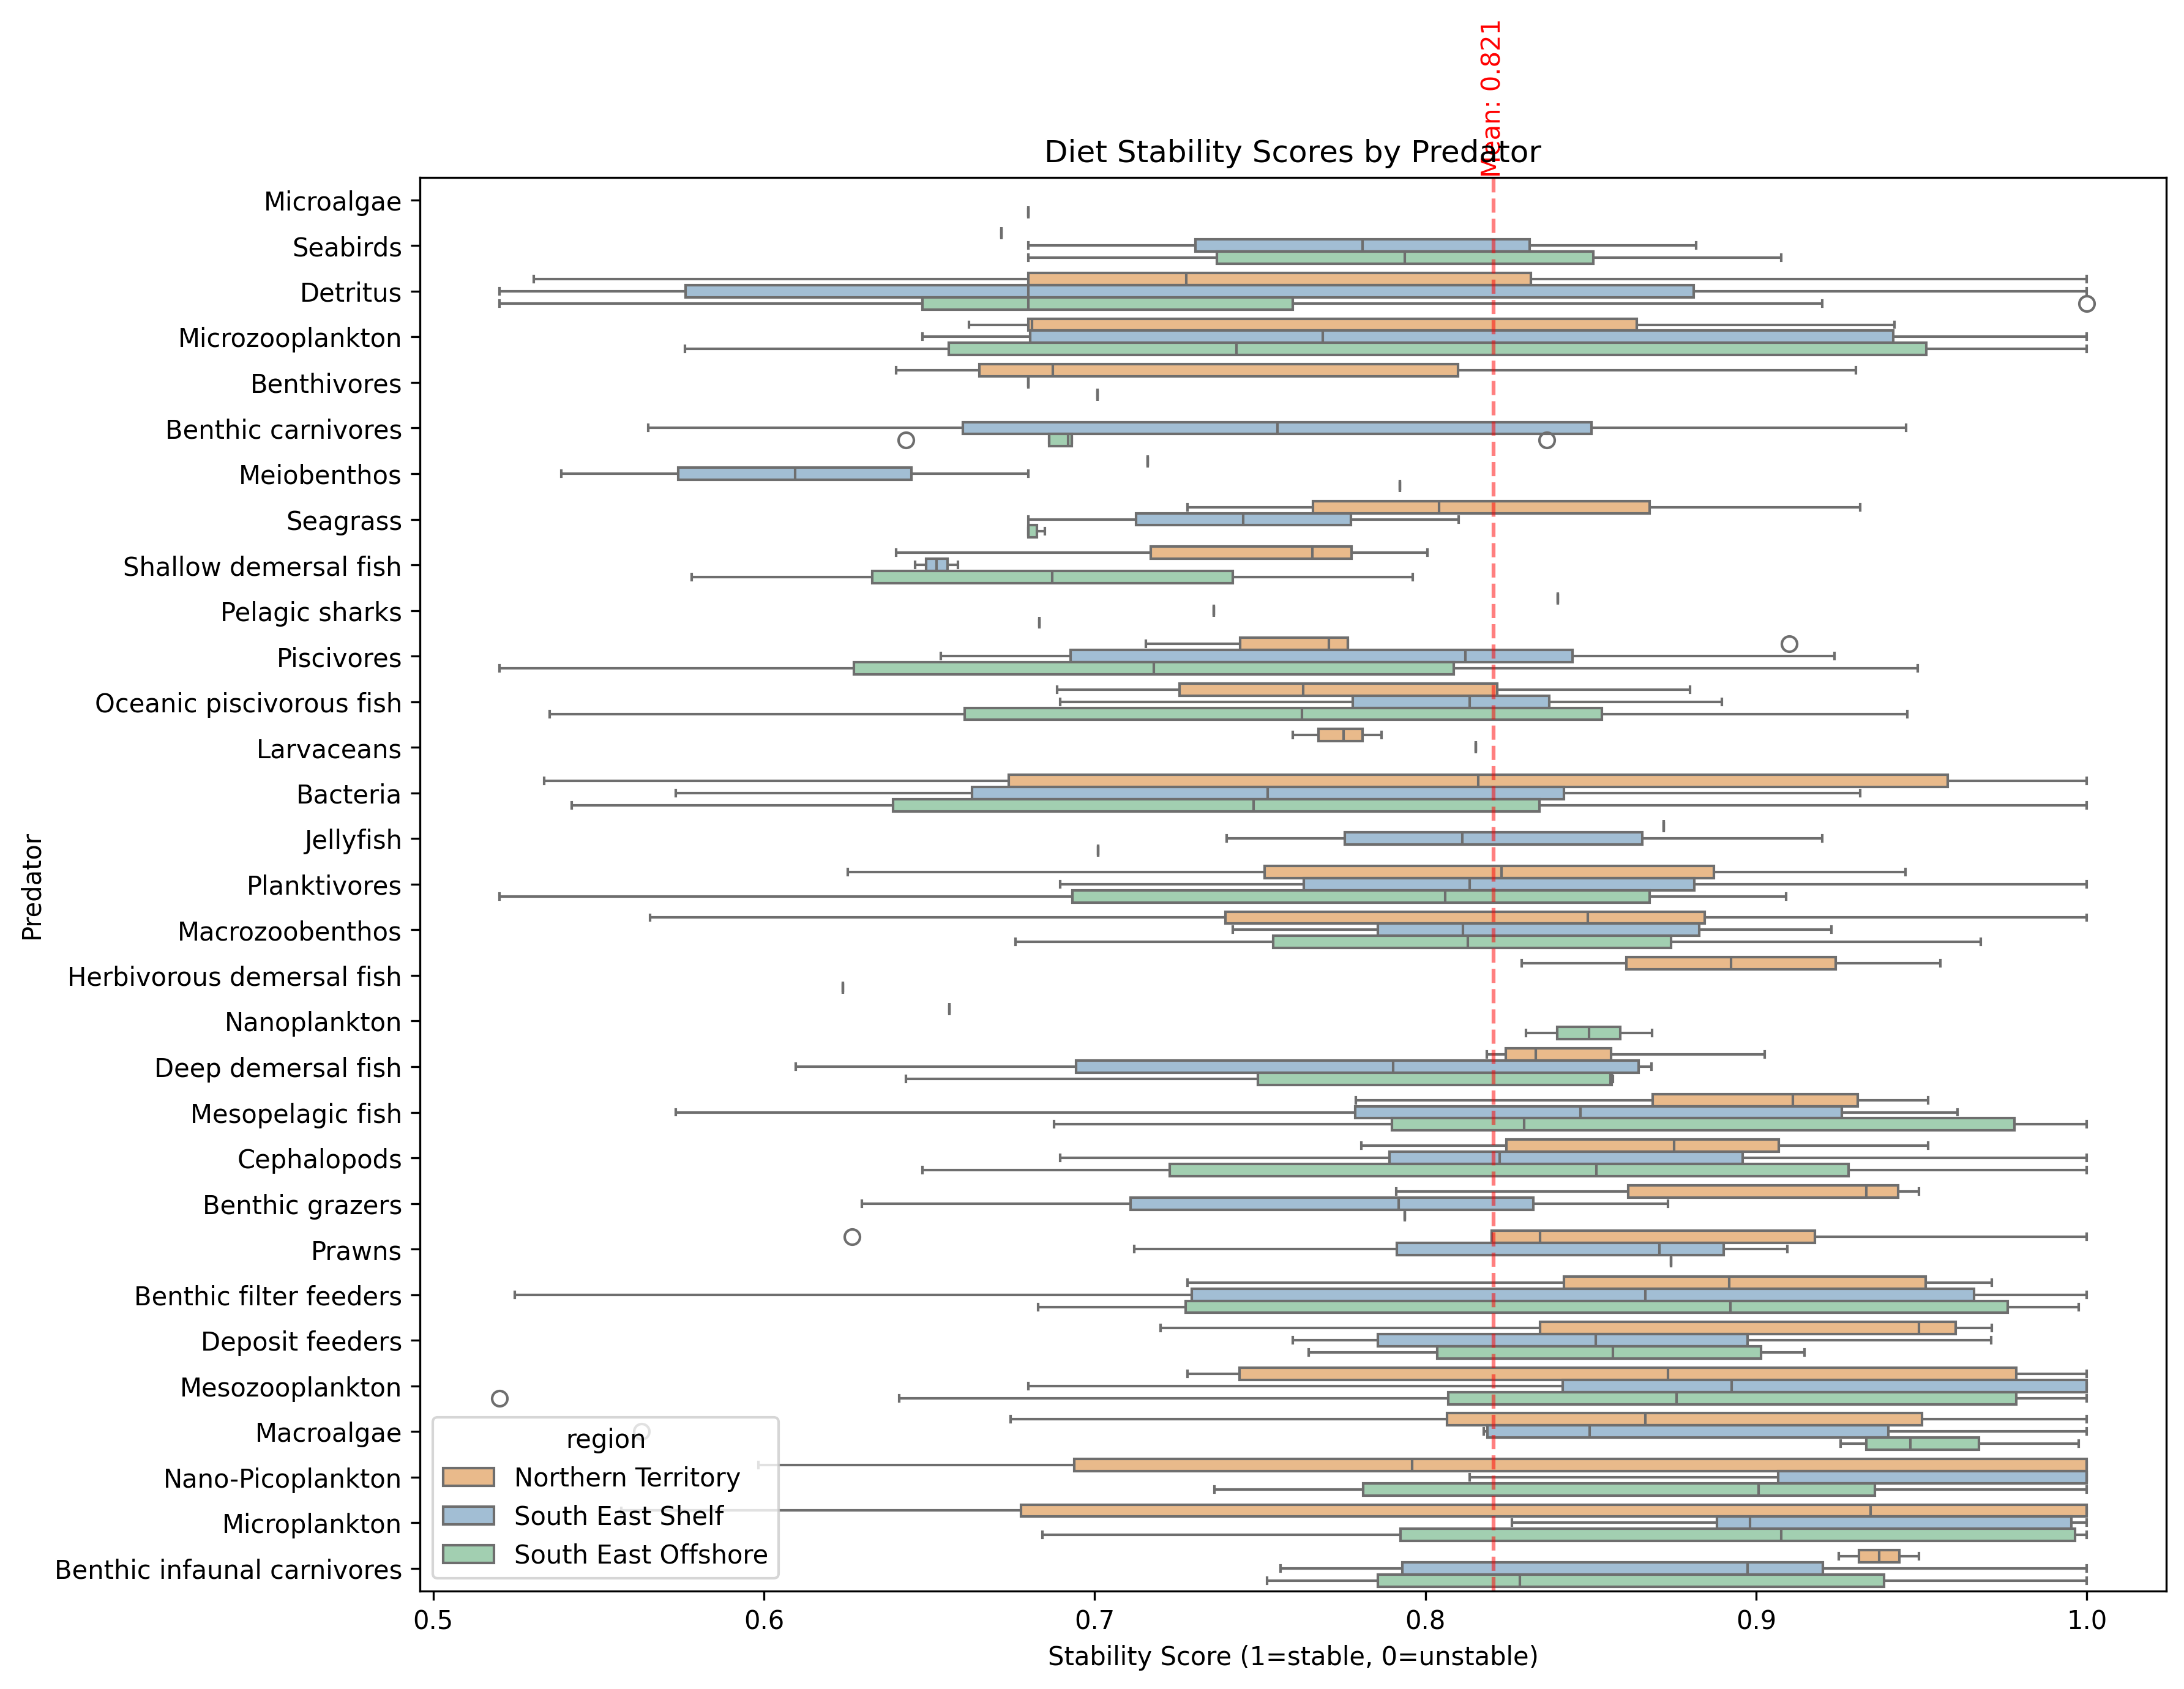
\includegraphics[width=\textwidth]{figures/predator_stability_boxplots.png}
  \caption{Diet stability scores for substantial interactions (those comprising more than 5\% of a predator's diet) grouped by predator, ordered by median stability. Box plots show the distribution of stability scores for each predator's diet across regions (colored by region). The red dashed line indicates the mean stability score across all included predator-prey interactions. Higher scores indicate more consistent diet compositions across framework iterations.}
  \label{fig:predator_stability}
\end{figure}



\suppsection{Technical Implementation}\label{supp:technical_implementation}
  \suppsubsection{Default Grouping with Descriptions}
  
  Table \ref{tab:functional_groups} presents the complete template of potential functional groups used by the system. This template serves as a reference for group classification, though the system can create new groups or modify existing ones based on specific ecosystem characteristics.
  
  \begin{longtable}{p{0.3\textwidth}p{0.7\textwidth}}
  \caption{Complete Functional Group Template\label{tab:functional_groups}} \\
  \hline
  \textbf{Group Name} & \textbf{Description} \\
  \hline
  \endfirsthead
  \multicolumn{2}{c}{{\tablename} \thetable{} -- Continued} \\
  \hline
  \textbf{Group Name} & \textbf{Description} \\
  \hline
  \endhead
  \hline
  \multicolumn{2}{r}{{Continued on next page}} \\
  \endfoot
  \hline
  \endlastfoot
  Skates and rays & Bottom-dwelling cartilaginous fish that play a role in controlling benthic prey populations \\
  Nearshore and smaller seabirds & Small gulls, terns etc that feed near shore (possibly include penguins here too) - avian predators that link marine and terrestrial ecosystems \\
  Albatrosses & Large seabirds that forage exclusively at sea, feeding on marine prey (fishes, squids, gelatinous organisms) \\
  Skuas and giant petrels & Large predatory seabirds that feed both at sea and on land, including predation on other birds \\
  Fish-eating pinnipeds & Marine mammals (seals, sea lions) that primarily prey on fish in coastal and pelagic ecosystems \\
  Invertebrate-eating pinnipeds & Marine mammals (particularly Antarctic seals) that primarily feed on krill and other invertebrates \\
  Baleen whales & Large filter-feeding marine mammals that regulate zooplankton populations and contribute to nutrient cycling \\
  Orcas & Apex predators that uniquely prey upon other top predators including marine mammals, sharks, and large fish \\
  Sperm whales & Deep-diving cetaceans that primarily feed on deep-water squid and fish \\
  Small toothed whales and dolphins & Smaller cetaceans that primarily feed on fish and squid in surface and mid-waters \\
  Sea snakes & Marine reptiles that prey primarily on fish, particularly eels and fish eggs \\
  Crocodiles & Large predatory reptiles in coastal and estuarine waters that prey on fish, birds, and mammals \\
  Turtles & Herbivores and omnivores that breed on land \\
  Planktivores & Small fishes that feed on plankton, crucial in transferring energy from plankton to larger predators \\
  Flying fish & Epipelagic fish capable of gliding above the water surface, important prey for many predators \\
  Remoras & Fish that form commensal relationships with larger marine animals, feeding on parasites and food scraps \\
  Large oceanic piscivorous fish & Fish-eating predators in open ocean environments, mid-sized non-migratory species (e.g. barracuda) \\
  Tuna and Billfish & Large oceanic predatory fish, highly mobile, often dive to feed deeper into the water column \\
  Shelf small benthivores & Small bodied fish that feed on benthic organisms, playing a key role in benthic-pelagic coupling, live in shelf waters \\
  Shelf demersal omnivorous fish & Medium sized demersal fish that feed on invertebrates as well as smaller fish, live in shelf waters \\
  Shelf medium demersal piscivores & Medium sized demersal fish living near the bottom in shallow waters, often important in benthic food webs, feed on other fish primarily, live in shelf waters \\
  Shelf large piscivores & Fish-eating predatory fishes found in various marine habitats, important in controlling prey fish populations \\
  Herbivorous demersal fish & Bottom-associated fish that primarily feed on plants, important in controlling algal growth \\
  Slope/deep water benthivores & Small to mid sized fish that feed on benthic organisms and live on the shelf or seamounts \\
  Slope/deep demersal omnivorous fish & Medium sized demersal fish that feed on invertebrates as well as smaller fish, live in slope or seamount waters \\
  Slope/deep medium demersal piscivores & Medium sized demersal fish that feed on other fish primarily, live in slope or seamount waters \\
  Slope/deep large piscivores & Fish-eating predatory fishes found in various marine habitats in deeper water, live in slope or seamount waters \\
  Migratory mesopelagic fish & Fish living in the mesopelagic zone, undertake diel vertical migration, important in energy transfer between depths \\
  Non-migratory mesopelagic fish & Fish living in the mesopelagic zone, non-migratory species, important in energy transfer between depths \\
  Reef sharks & Top predators in coral reef ecosystems, controlling fish populations and maintaining reef health \\
  Pelagic sharks & Open-ocean predators that help regulate populations of fishes and squids \\
  Demersal sharks & Bottom-dwelling sharks, including dogfishes, that control populations of fishes and invertebrates on and near the seafloor \\
  Cephalopods & Intelligent mollusks like squid and octopus, important predators in many marine ecosystems \\
  Hard corals & Reef-building colonial animals that create complex habitat structure through calcium carbonate deposition \\
  Soft corals & Colonial animals that contribute to reef habitat complexity without building calcium carbonate structures \\
  Sea anemones & Predatory anthozoans that can form symbiotic relationships with fish and crustaceans \\
  Hydrothermal vent communities & Specialized organisms living around deep-sea vents, including chemosynthetic bacteria and associated fauna \\
  Cold seep communities & Organisms adapted to methane and sulfide-rich environments on the seafloor \\
  Deep-sea glass sponges & Filter-feeding animals that create complex deep-water habitats and are important in silicon cycling \\
  Sea cucumbers & Deposit-feeding echinoderms important in sediment processing and bioturbation \\
  Sea urchins & Herbivorous echinoderms that can control macroalgal abundance and affect reef structure \\
  Crown-of-thorns starfish & Coral-eating sea stars that can significantly impact reef health during population outbreaks \\
  Benthic filter feeders & Bottom-dwelling organisms that filter water for food, important in nutrient cycling and regulating water quality in various depths - bivalves, crinoids, sponges \\
  Macrozoobenthos & Mobile large bottom-dwelling invertebrates in both shallow and deep waters, important in benthic food webs and bioturbation (predatory or omnivorous) \\
  Benthic grazers & Bottom-dwelling organisms that graze on algae and detritus, influencing benthic community structure \\
  Prawns & Small crustaceans that are important in benthic and pelagic food webs \\
  Meiobenthos & Tiny bottom-dwelling organisms, important in sediment processes and as food for larger animals \\
  Deposit feeders & Animals that feed on organic matter in sediments, important in nutrient cycling \\
  Benthic infaunal carnivores & Predatory animals living within the seafloor sediments \\
  Sedimentary Bacteria & Microscopic organisms crucial in nutrient cycling and the microbial loop in marine ecosystems \\
  Large carnivorous zooplankton & Fish larvae, arrow worms and other large predatory zooplankton \\
  Antarctic krill & Key species in Antarctic food webs, particularly important as prey for whales, seals, and seabirds \\
  Ice-associated algae & Microalgae living within and on the underside of sea ice, important primary producers in polar regions \\
  Ice-associated fauna & Specialized invertebrates living in association with sea ice, important in polar food webs \\
  Mesozooplankton & Medium-sized zooplankton (200 µm to 2 cm) that feed on smaller plankton and serve as food for larger animals \\
  Microzooplankton & Tiny zooplankton (20 µm to 200 µm) that graze on phytoplankton and bacteria, forming a crucial link in the microbial food web \\
  Pelagic tunicates & Including larvaceans, salps, and pyrosomes, important in marine snow formation and carbon cycling \\
  Jellyfish & Predatory gelatinous species \\
  Diatoms & Larger phytoplankton (20 µm to 200 µm), silica dependent important primary producers in marine ecosystems \\
  Dinoflagellates & Mixotrophic species (20 µm to 200 µm) that can switch between primary production and consumption as needed \\
  Nanoplankton & Plankton ranging from 2 µm to 20 µm in size, including small algae and protozoans \\
  Picoplankton & Plankton ranging from 0.2 µm to 2 µm in size, including both photosynthetic and heterotrophic organisms \\
  Microalgae (microphytobenthos) & Microscopic algae that live on the seafloor or attached to other organisms \\
  Pelagic bacteria & Watercolumn dwelling bacteria, consume marine snow amongst other things \\
  Seagrass & Marine flowering plants that form important coastal habitats and nursery areas \\
  Mangroves & Salt-tolerant trees forming critical coastal nursery habitats and protecting shorelines \\
  Salt marsh plants & Coastal vegetation adapted to periodic flooding, important in nutrient cycling and shoreline protection \\
  Macroalgae & Seaweeds of various sizes that provide habitat and food for many species, including both canopy and understory forms \\
  Symbiotic zooxanthellae & Photosynthetic dinoflagellates living within coral and other marine invertebrates \\
  Cleaner fish and shrimp & Species that remove parasites from other marine animals, important in reef health \\
  Discards & Carrion and freshly discarded material from fisheries activities \\
  Detritus & Labile components of natural death and waste \\
  \end{longtable}
  
  \suppsubsection{Retrieval-Augmented Generation Implementation}\label{supp:rag_implementation}
  
  We implement a retrieval-augmented generation system using ChromaDB for vector storage and document management. Document processing begins with LlamaParse conversion of source materials to markdown format, preserving structural elements while enabling consistent text extraction across document types. We segment documents using a token-aware chunking strategy with a 2000-token maximum size, determined through empirical testing to balance context preservation with model limitations.
  
  Document processing follows a two-phase approach. The initial phase generates embeddings for each document chunk using Azure OpenAI's text-embedding-3-small model, storing them in ChromaDB's PersistentClient. The system maintains an indexed\_files.json registry to track processed documents. The second phase handles incremental updates, identifying and processing only new content when documents are added to the source directory.
  
  For diet composition analysis, we implement a two-stage query process. The first stage employs a simple query to retrieve relevant document chunks:
  
  \begin{prompt}
  What do [group] eat?
  \end{prompt}
  
  The system embeds this query using the same Azure OpenAI model and performs vector similarity search to identify relevant document chunks. These results combine with structured data sources including species occurrence frequencies, food category classifications, and GLOBI interaction data to form a comprehensive input for the second stage.
  
  We implement comprehensive error handling throughout the pipeline. The system employs exponential backoff retry logic for API interactions, with configurable parameters including maximum retries (10), initial delay (1 second), and maximum delay (300 seconds). For model interactions, we utilise LlamaIndex's query engine with zero-temperature sampling to ensure deterministic responses. The system supports multiple language model backends including Claude-3 Sonnet (200k token context), GPT-4, and AWS Claude, enabling flexible deployment based on availability and performance requirements.
  
  The system maintains separate storage contexts for different document collections through ChromaDB's collection management. This separation prevents cross-contamination between knowledge bases while enabling efficient parallel processing. We track document citations throughout the retrieval process, maintaining provenance information for all retrieved content. The complete implementation, including embedding generation, chunking algorithms, and query processing functions, is available in the project repository.
